\section{从无前缀安全PRF到完全安全PRF(方法1):加密PRF}\label{sec:6-5}

我们下面展示如何将无前缀安全的 PRF $F_{\rm CBC}$ 和 $F^*$ 转换为安全的 PRF,这将为我们提供针对变长输入的安全 MAC。更一般地,我们将展示如何将无前缀安全的 PRF $PF$ 转换为完全安全的 PRF。我们会介绍以下三种方法:
\begin{itemize}
	\item 加密 PRF:用另一个 PRF 对 $PF$ 的短输出进行加密。
	\item 无前缀编码:对 $PF$ 的输入进行编码,使得任意一个输入都不是其他输入的前缀。
	\item CMAC:引入随机化的一种更有效的无前缀编码。
\end{itemize}
在这一节中,我们首先介绍加密 PRF 的方法。这个构造是相当直接的。令 PF 是一个从 $\mathcal{X}^{\leq\ell}$ 映射到 $\mathcal{Y}$ 的 PRF,$F$ 是一个从 $\mathcal{Y}$ 映射到 $\mathcal{T}$ 的 PRF。定义:
\begin{equation}\label{eq:6-17}
EF\big((k_1,k_2),\;m\big)=F\big(k_2,\;PF(k_1,m)\big)
\end{equation}
该构造如图 \ref{fig:6-4} 所示。

\begin{figure}
  \centering
%  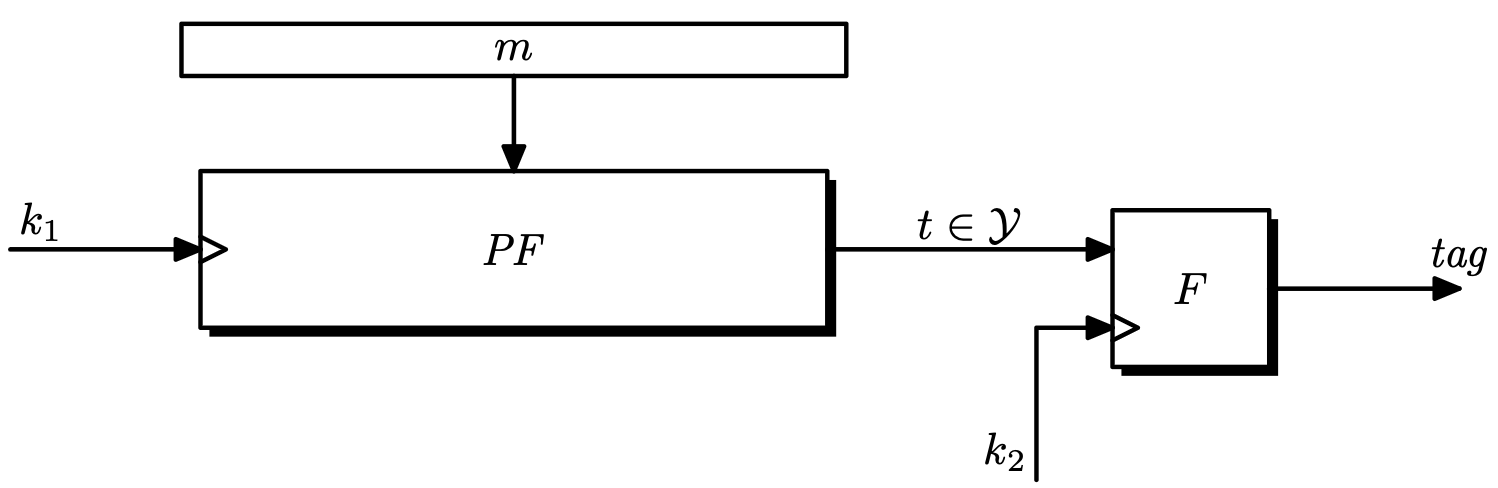
\includegraphics[width=0.65\linewidth]{figures/chapter6/fig4.png}
  \tikzset{every picture/.style={line width=0.75pt}} %set default line width to 0.75pt        

\begin{tikzpicture}[x=0.75pt,y=0.75pt,yscale=-1,xscale=1]
%uncomment if require: \path (0,160); %set diagram left start at 0, and has height of 160

%Shape: Rectangle [id:dp33326858691181327] 
\draw  [fill={rgb, 255:red, 255; green, 255; blue, 255 }  ,fill opacity=1 ][line width=1.2]  (50,0) -- (230,0) -- (230,20) -- (50,20) -- cycle ;
%Shape: Rectangle [id:dp083961736493265] 
\draw  [fill={rgb, 255:red, 255; green, 255; blue, 255 }  ,fill opacity=1 ][line width=1.2] [general shadow={fill=black,shadow xshift=2.25pt,shadow yshift=-2.25pt}] (300,60) -- (350,60) -- (350,110) -- (300,110) -- cycle ;
%Straight Lines [id:da7095405239206141] 
\draw    (350,85) -- (397,85) ;
\draw [shift={(400,85)}, rotate = 180] [fill={rgb, 255:red, 0; green, 0; blue, 0 }  ][line width=0.08]  [draw opacity=0] (7.14,-3.43) -- (0,0) -- (7.14,3.43) -- cycle    ;
%Straight Lines [id:da9545512828776872] 
\draw    (0,75) -- (47,75) ;
\draw [shift={(50,75)}, rotate = 180] [fill={rgb, 255:red, 0; green, 0; blue, 0 }  ][line width=0.08]  [draw opacity=0] (7.14,-3.43) -- (0,0) -- (7.14,3.43) -- cycle    ;
%Straight Lines [id:da15363507283754263] 
\draw    (140,20) -- (140,47) ;
\draw [shift={(140,50)}, rotate = 270] [fill={rgb, 255:red, 0; green, 0; blue, 0 }  ][line width=0.08]  [draw opacity=0] (7.14,-3.43) -- (0,0) -- (7.14,3.43) -- cycle    ;
%Straight Lines [id:da3074642964706582] 
\draw    (275,140) -- (275,95) -- (297,95) ;
\draw [shift={(300,95)}, rotate = 180] [fill={rgb, 255:red, 0; green, 0; blue, 0 }  ][line width=0.08]  [draw opacity=0] (7.14,-3.43) -- (0,0) -- (7.14,3.43) -- cycle    ;
%Flowchart: Extract [id:dp5425750567919283] 
\draw   (305,95) -- (300,98.5) -- (300,91.5) -- cycle ;
%Shape: Rectangle [id:dp7127919566797498] 
\draw  [fill={rgb, 255:red, 255; green, 255; blue, 255 }  ,fill opacity=1 ][line width=1.2] [general shadow={fill=black,shadow xshift=2.25pt,shadow yshift=-2.25pt}] (50,50) -- (230,50) -- (230,100) -- (50,100) -- cycle ;
%Flowchart: Extract [id:dp7415383977392733] 
\draw   (55,75) -- (50,78.5) -- (50,71.5) -- cycle ;
%Straight Lines [id:da7132747696931903] 
\draw    (230,75) -- (297,75) ;
\draw [shift={(300,75)}, rotate = 180] [fill={rgb, 255:red, 0; green, 0; blue, 0 }  ][line width=0.08]  [draw opacity=0] (7.14,-3.43) -- (0,0) -- (7.14,3.43) -- cycle    ;

% Text Node
\draw (325,85) node    {$F$};
% Text Node
\draw (140,10) node    {$m$};
% Text Node
\draw (400,81.6) node [anchor=south] [inner sep=0.75pt]    {$tag$};
% Text Node
\draw (2,71.6) node [anchor=south west] [inner sep=0.75pt]    {$k_{1}$};
% Text Node
\draw (140,75) node    {$PF$};
% Text Node
\draw (265,71.6) node [anchor=south] [inner sep=0.75pt]    {$t\in \mathcal{Y}$};
% Text Node
\draw (273,136.6) node [anchor=south east] [inner sep=0.75pt]    {$k_{2}$};


\end{tikzpicture}
  \caption{加密 PRF 构造 $EF(k,m)$}
  \label{fig:6-4}
\end{figure}

我们声称,当 $PF$ 是 CBC 或级联中的任何一种构造时,$EF$ 都是一个安全的 PRF。更一般地,我们表明,只要 $PF$ 是一个\emph{可扩展的} PRF,$EF$ 就是安全的。可扩展性的定义如下:

\begin{definition}\label{def:6-4}
令 $PF$ 是一个定义在 $(\mathcal{K},\mathcal{X}^{\leq\ell},\mathcal{Y})$ 上的 PRF。如果对于所有的 $k\in\mathcal{K}$,$x,y\in\mathcal{X}^{\leq\ell-1}$ 和 $a\in\mathcal{X}$,我们都有:
\[
\text{if}\quad
PF(k,x)=PF(k,y)
\quad\text{then}\quad
PF(k,\;x\,\Vert\,a)=PF(k,\;y\,\Vert\,a)
\]
就称 $PF$ 是一个\textbf{可扩展 (extendable) PRF}。
\end{definition}

不难发现,CBC 和级联构造都是可扩展的 PRF。下面的定理将表明,如果 $PF$ 是一个可扩展的无前缀安全 PRF,$EF$ 就是一个安全的 PRF。

\begin{theorem}\label{theo:6-5}
令 $PF$ 是一个定义在 $(\mathcal{K}_1,\mathcal{X}^{\leq\ell+1},\mathcal{Y})$ 上的可扩展且无前缀安全的 PRF,其中 $|\mathcal{Y}|$ 是超多项式的,$\ell$ 是多项式约束的。令 $F$ 是一个定义在 $(\mathcal{K}_2,\mathcal{Y},\mathcal{T})$ 上的安全的 PRF。那么如式 \ref{eq:6-17} 中所定义的 $EF$ 是一个定义在 $(\mathcal{K}_1\times\mathcal{K}_2,\mathcal{X}^{\leq\ell},\mathcal{T})$ 上的安全的 PRF。
\begin{quote}
特别地,对于每个按照攻击游戏 \ref{game:4-2} 攻击 $EF$ 的 PRF 对手 $\mathcal{A}$,假设它最多能够向其挑战者发起 $Q$ 次查询,则必然存在一个按照攻击游戏 \ref{game:4-2} 攻击 $F$ 的 PRF 对手 $\mathcal{B}_1$ 和一个按照攻击游戏 \ref{game:4-2} 攻击 $PF$ 的无前缀 PRF 对手 $\mathcal{B}_2$,其中 $\mathcal{B}_1$ 和 $\mathcal{B}_2$ 都是围绕 $\mathcal{A}$ 的基本包装器,满足:
\end{quote}
\begin{equation}\label{eq:6-18}
{\rm PRF\mathsf{adv}}[\mathcal{A},EF]\leq {\rm PRF\mathsf{adv}}[\mathcal{B}_1,F]+{\rm PRF^{pf}\mathsf{adv}}[\mathcal{B}_2,PF]+\frac{Q^2}{2|\mathcal{Y}|}
\end{equation}
\end{theorem}

\noindent
在我们提供了必要的工具之后,我们将在下一章(\ref{subsec:7-3-1} 小节)证明定理 \ref{theo:6-5}。请注意,为了使 $EF$ 在长度不超过 $\ell$ 的输入上都是安全的 PRF,该定理要求 $PF$ 对于长为 $\ell+1$ 的输入是都无前缀安全的。

\begin{snote}[式 \ref{eq:6-18} 中的上界是严格的。]
虽然不是完全必要,但让我们假设 $\mathcal{Y}=\mathcal{T}$,$F$ 是一个分组密码,并且 $|\mathcal{X}|$ 不是非常小。这些假设将大大简化论证。我们下面展示一种攻击,它能在 $Q\approx\sqrt{|\mathcal{Y}|}$ 次查询之后以恒定概率攻破 $EF$。事实上,我们的攻击将攻破作为一个 MAC 的 $EF$。对手首先挑选 $Q$ 个随机输入 $x_1,\dots,x_Q\in\mathcal{X}^2$,并用这 $Q$ 个输入向其挑战者发起查询,以得到应答 $t_1,\dots,t_Q\in\mathcal{T}$。根据生日悖论(推论 \ref{cor:B-2}),对于任何固定的密钥 $k_1$,存在不同的索引 $i$ 和 $j$ 使得 $x_i\neq x_j$ 且 $PF(k_1,x_i)=PF(k_1,x_j)$ 的概率是恒定的。一方面,如果发生这样的碰撞,我们可以有效发现它,这是因为对于这样的一对索引,必有 $t_i=t_j$。另一方面,如果存在一对索引 $i$ 和 $j$ 使得 $t_i=t_j$,由于我们假设 $F$ 是一个分组密码,那么必然有 $PF(k_1,x_i)=PF(k_1,x_j)$。现在,假设 $x_i\neq x_j$ 且 $PF(k_1,x_i)=PF(k_1,x_j)$,由于 $PF$ 是可扩展的,那么对于任意 $a\in\mathcal{X}$,我们都有 $PF\big(k_1,\,(x_i\,\Vert\,a)\big)=PF\big(k_1,\,(x_j\,\Vert\,a)\big)$。因此,我们的对手可以获得 $x_i\,\Vert\,a$ 的 MAC 标签 $t$,而这个标签 $t$ 同时也是 $x_j\,\Vert\,a$ 的有效标签。推广这一攻击,我们就能很容易地证明式 \ref{eq:6-18} 中 ${Q^2}/{(2|\mathcal{Y}|)}$ 这一项的必要性。
\end{snote}

\subsection{ECBC 和 NMAC:用于变长输入的安全 PRF}\label{subsec:6-5-1}

图 \ref{fig:6-5-a} 和 \ref{fig:6-5-b} 展示了对 CBC 和级联应用 $EF$ 构造的结果。

\begin{figure}
  \centering
  \subfigure[ECBC 构造 $\mathrm{ECBC}(k,m)$(加密CBC)]{
    

\tikzset{every picture/.style={line width=0.75pt}} %set default line width to 0.75pt        

\begin{tikzpicture}[x=0.75pt,y=0.75pt,yscale=-1,xscale=1]
%uncomment if require: \path (0,181); %set diagram left start at 0, and has height of 181

%Shape: Rectangle [id:dp4443145165233573] 
\draw  [fill={rgb, 255:red, 255; green, 255; blue, 255 }  ,fill opacity=1 ][line width=1.2] [general shadow={fill=black,shadow xshift=2.25pt,shadow yshift=-2.25pt}] (10,90) -- (60,90) -- (60,140) -- (10,140) -- cycle ;
%Shape: Rectangle [id:dp3654823418270836] 
\draw  [fill={rgb, 255:red, 255; green, 255; blue, 255 }  ,fill opacity=1 ][line width=1.2] [general shadow={fill=black,shadow xshift=2.25pt,shadow yshift=-2.25pt}] (0,0) -- (70,0) -- (70,20) -- (0,20) -- cycle ;
%Shape: Rectangle [id:dp893088791780835] 
\draw  [fill={rgb, 255:red, 255; green, 255; blue, 255 }  ,fill opacity=1 ][line width=1.2] [general shadow={fill=black,shadow xshift=2.25pt,shadow yshift=-2.25pt}] (100,0) -- (170,0) -- (170,20) -- (100,20) -- cycle ;
%Shape: Rectangle [id:dp4783618167357453] 
\draw  [fill={rgb, 255:red, 255; green, 255; blue, 255 }  ,fill opacity=1 ][line width=1.2] [general shadow={fill=black,shadow xshift=2.25pt,shadow yshift=-2.25pt}] (200,0) -- (270,0) -- (270,20) -- (200,20) -- cycle ;
%Shape: Rectangle [id:dp14886948130262612] 
\draw  [fill={rgb, 255:red, 255; green, 255; blue, 255 }  ,fill opacity=1 ][line width=1.2] [general shadow={fill=black,shadow xshift=2.25pt,shadow yshift=-2.25pt}] (330,0) -- (400,0) -- (400,20) -- (330,20) -- cycle ;
%Shape: Rectangle [id:dp8119610043743812] 
\draw  [fill={rgb, 255:red, 255; green, 255; blue, 255 }  ,fill opacity=1 ][line width=1.2] [general shadow={fill=black,shadow xshift=2.25pt,shadow yshift=-2.25pt}] (110,90) -- (160,90) -- (160,140) -- (110,140) -- cycle ;
%Shape: Rectangle [id:dp18004760511222906] 
\draw  [fill={rgb, 255:red, 255; green, 255; blue, 255 }  ,fill opacity=1 ][line width=1.2] [general shadow={fill=black,shadow xshift=2.25pt,shadow yshift=-2.25pt}] (210,90) -- (260,90) -- (260,140) -- (210,140) -- cycle ;
%Shape: Rectangle [id:dp960423359685666] 
\draw  [fill={rgb, 255:red, 255; green, 255; blue, 255 }  ,fill opacity=1 ][line width=1.2] [general shadow={fill=black,shadow xshift=2.25pt,shadow yshift=-2.25pt}] (340,90) -- (390,90) -- (390,140) -- (340,140) -- cycle ;
%Straight Lines [id:da44373949352543574] 
\draw    (35,20) -- (35,87) ;
\draw [shift={(35,90)}, rotate = 270] [fill={rgb, 255:red, 0; green, 0; blue, 0 }  ][line width=0.08]  [draw opacity=0] (7.14,-3.43) -- (0,0) -- (7.14,3.43) -- cycle    ;
%Straight Lines [id:da38045035541987127] 
\draw    (60,115) -- (85,115) -- (85,55) -- (127,55) ;
\draw [shift={(130,55)}, rotate = 180] [fill={rgb, 255:red, 0; green, 0; blue, 0 }  ][line width=0.08]  [draw opacity=0] (7.14,-3.43) -- (0,0) -- (7.14,3.43) -- cycle    ;
%Straight Lines [id:da6694268861945114] 
\draw    (160,115) -- (185,115) -- (185,55) -- (227,55) ;
\draw [shift={(230,55)}, rotate = 180] [fill={rgb, 255:red, 0; green, 0; blue, 0 }  ][line width=0.08]  [draw opacity=0] (7.14,-3.43) -- (0,0) -- (7.14,3.43) -- cycle    ;
%Straight Lines [id:da1731188178152383] 
\draw    (330,55) -- (357,55) ;
\draw [shift={(360,55)}, rotate = 180] [fill={rgb, 255:red, 0; green, 0; blue, 0 }  ][line width=0.08]  [draw opacity=0] (7.14,-3.43) -- (0,0) -- (7.14,3.43) -- cycle    ;
%Straight Lines [id:da18974241223755217] 
\draw    (135,20) -- (135,47) ;
\draw [shift={(135,50)}, rotate = 270] [fill={rgb, 255:red, 0; green, 0; blue, 0 }  ][line width=0.08]  [draw opacity=0] (7.14,-3.43) -- (0,0) -- (7.14,3.43) -- cycle    ;
%Straight Lines [id:da9241213725477959] 
\draw    (135,60) -- (135,87) ;
\draw [shift={(135,90)}, rotate = 270] [fill={rgb, 255:red, 0; green, 0; blue, 0 }  ][line width=0.08]  [draw opacity=0] (7.14,-3.43) -- (0,0) -- (7.14,3.43) -- cycle    ;
%Straight Lines [id:da8064891185926979] 
\draw    (235,20) -- (235,47) ;
\draw [shift={(235,50)}, rotate = 270] [fill={rgb, 255:red, 0; green, 0; blue, 0 }  ][line width=0.08]  [draw opacity=0] (7.14,-3.43) -- (0,0) -- (7.14,3.43) -- cycle    ;
%Straight Lines [id:da20365370380672698] 
\draw    (365,20) -- (365,47) ;
\draw [shift={(365,50)}, rotate = 270] [fill={rgb, 255:red, 0; green, 0; blue, 0 }  ][line width=0.08]  [draw opacity=0] (7.14,-3.43) -- (0,0) -- (7.14,3.43) -- cycle    ;
%Straight Lines [id:da8209148833770106] 
\draw    (235,60) -- (235,87) ;
\draw [shift={(235,90)}, rotate = 270] [fill={rgb, 255:red, 0; green, 0; blue, 0 }  ][line width=0.08]  [draw opacity=0] (7.14,-3.43) -- (0,0) -- (7.14,3.43) -- cycle    ;
%Straight Lines [id:da41897506139568685] 
\draw    (365,60) -- (365,87) ;
\draw [shift={(365,90)}, rotate = 270] [fill={rgb, 255:red, 0; green, 0; blue, 0 }  ][line width=0.08]  [draw opacity=0] (7.14,-3.43) -- (0,0) -- (7.14,3.43) -- cycle    ;
%Straight Lines [id:da5786817284582193] 
\draw    (260,115) -- (285,115) ;
%Straight Lines [id:da354850726992592] 
\draw  [dash pattern={on 0.84pt off 2.51pt}]  (285,115) -- (310,115) -- (310,55) -- (330,55) ;
%Straight Lines [id:da7935744551156634] 
\draw    (490,115) -- (537,115) ;
\draw [shift={(540,115)}, rotate = 180] [fill={rgb, 255:red, 0; green, 0; blue, 0 }  ][line width=0.08]  [draw opacity=0] (7.14,-3.43) -- (0,0) -- (7.14,3.43) -- cycle    ;
%Shape: Rectangle [id:dp5498562140150316] 
\draw  [fill={rgb, 255:red, 255; green, 255; blue, 255 }  ,fill opacity=1 ][line width=1.2] [general shadow={fill=black,shadow xshift=2.25pt,shadow yshift=-2.25pt}] (440,90) -- (490,90) -- (490,140) -- (440,140) -- cycle ;
%Straight Lines [id:da297515876064387] 
\draw    (390,115) -- (437,115) ;
\draw [shift={(440,115)}, rotate = 180] [fill={rgb, 255:red, 0; green, 0; blue, 0 }  ][line width=0.08]  [draw opacity=0] (7.14,-3.43) -- (0,0) -- (7.14,3.43) -- cycle    ;
%Straight Lines [id:da29951358036034725] 
\draw  [dash pattern={on 4.5pt off 4.5pt}]  (0,165) -- (400,165) ;
\draw [shift={(400,165)}, rotate = 180] [color={rgb, 255:red, 0; green, 0; blue, 0 }  ][line width=0.75]    (0,4.47) -- (0,-4.47)   ;
\draw [shift={(0,165)}, rotate = 180] [color={rgb, 255:red, 0; green, 0; blue, 0 }  ][line width=0.75]    (0,4.47) -- (0,-4.47)   ;
%Shape: Rectangle [id:dp3234507369689261] 
\draw  [draw opacity=0][fill={rgb, 255:red, 255; green, 255; blue, 255 }  ,fill opacity=1 ] (175,155) -- (225,155) -- (225,175) -- (175,175) -- cycle ;

% Text Node
\draw (35,115) node    {$F( k_{1} ,\cdot )$};
% Text Node
\draw (135,115) node    {$F( k_{1} ,\cdot )$};
% Text Node
\draw (235,115) node    {$F( k_{1} ,\cdot )$};
% Text Node
\draw (365,115) node    {$F( k_{1} ,\cdot )$};
% Text Node
\draw (135,55) node  [font=\large]  {$\oplus $};
% Text Node
\draw (235,55) node  [font=\large]  {$\oplus $};
% Text Node
\draw (365,55) node  [font=\large]  {$\oplus $};
% Text Node
\draw (300,10) node    {$\cdots $};
% Text Node
\draw (35,10) node    {$a_{1}$};
% Text Node
\draw (135,10) node    {$a_{2}$};
% Text Node
\draw (235,10) node    {$a_{3}$};
% Text Node
\draw (365,10) node    {$a_{\ell }$};
% Text Node
\draw (540,111.6) node [anchor=south] [inner sep=0.75pt]    {$tag$};
% Text Node
\draw (465,115) node    {$F( k_{2} ,\cdot )$};
% Text Node
\draw (200,165) node   [align=left] {CBC};


\end{tikzpicture}
  	\label{fig:6-5-a}
  }
  
  \,
  
  \,
  
  \subfigure[NMAC 构造 $\mathrm{NMAC}(k,m)$(加密级联)]{
  	

\tikzset{every picture/.style={line width=0.75pt}} %set default line width to 0.75pt        

\begin{tikzpicture}[x=0.75pt,y=0.75pt,yscale=-1,xscale=1]
%uncomment if require: \path (0,182); %set diagram left start at 0, and has height of 182

%Shape: Rectangle [id:dp8247531494470199] 
\draw  [fill={rgb, 255:red, 255; green, 255; blue, 255 }  ,fill opacity=1 ][line width=1.2] [general shadow={fill=black,shadow xshift=2.25pt,shadow yshift=-2.25pt}] (50,50) -- (100,50) -- (100,100) -- (50,100) -- cycle ;
%Shape: Rectangle [id:dp6129441991681601] 
\draw  [fill={rgb, 255:red, 255; green, 255; blue, 255 }  ,fill opacity=1 ][line width=1.2] [general shadow={fill=black,shadow xshift=2.25pt,shadow yshift=-2.25pt}] (40,0) -- (110,0) -- (110,20) -- (40,20) -- cycle ;
%Shape: Rectangle [id:dp90829523247659] 
\draw  [fill={rgb, 255:red, 255; green, 255; blue, 255 }  ,fill opacity=1 ][line width=1.2] [general shadow={fill=black,shadow xshift=2.25pt,shadow yshift=-2.25pt}] (140,0) -- (210,0) -- (210,20) -- (140,20) -- cycle ;
%Shape: Rectangle [id:dp08202625686221188] 
\draw  [fill={rgb, 255:red, 255; green, 255; blue, 255 }  ,fill opacity=1 ][line width=1.2] [general shadow={fill=black,shadow xshift=2.25pt,shadow yshift=-2.25pt}] (270,0) -- (340,0) -- (340,20) -- (270,20) -- cycle ;
%Shape: Rectangle [id:dp9192770861603901] 
\draw  [fill={rgb, 255:red, 255; green, 255; blue, 255 }  ,fill opacity=1 ][line width=1.2] [general shadow={fill=black,shadow xshift=2.25pt,shadow yshift=-2.25pt}] (150,50) -- (200,50) -- (200,100) -- (150,100) -- cycle ;
%Shape: Rectangle [id:dp6226214384270212] 
\draw  [fill={rgb, 255:red, 255; green, 255; blue, 255 }  ,fill opacity=1 ][line width=1.2] [general shadow={fill=black,shadow xshift=2.25pt,shadow yshift=-2.25pt}] (280,50) -- (330,50) -- (330,100) -- (280,100) -- cycle ;
%Straight Lines [id:da593286075335618] 
\draw    (100,75) -- (147,75) ;
\draw [shift={(150,75)}, rotate = 180] [fill={rgb, 255:red, 0; green, 0; blue, 0 }  ][line width=0.08]  [draw opacity=0] (7.14,-3.43) -- (0,0) -- (7.14,3.43) -- cycle    ;
%Straight Lines [id:da362450281296391] 
\draw    (175,20) -- (175,47) ;
\draw [shift={(175,50)}, rotate = 270] [fill={rgb, 255:red, 0; green, 0; blue, 0 }  ][line width=0.08]  [draw opacity=0] (7.14,-3.43) -- (0,0) -- (7.14,3.43) -- cycle    ;
%Straight Lines [id:da04154463636417449] 
\draw    (305,20) -- (305,47) ;
\draw [shift={(305,50)}, rotate = 270] [fill={rgb, 255:red, 0; green, 0; blue, 0 }  ][line width=0.08]  [draw opacity=0] (7.14,-3.43) -- (0,0) -- (7.14,3.43) -- cycle    ;
%Straight Lines [id:da932866823555605] 
\draw    (330,75) -- (397,75) ;
\draw [shift={(400,75)}, rotate = 180] [fill={rgb, 255:red, 0; green, 0; blue, 0 }  ][line width=0.08]  [draw opacity=0] (7.14,-3.43) -- (0,0) -- (7.14,3.43) -- cycle    ;
%Straight Lines [id:da5223337867158735] 
\draw    (0,75) -- (47,75) ;
\draw [shift={(50,75)}, rotate = 180] [fill={rgb, 255:red, 0; green, 0; blue, 0 }  ][line width=0.08]  [draw opacity=0] (7.14,-3.43) -- (0,0) -- (7.14,3.43) -- cycle    ;
%Straight Lines [id:da7098873699377382] 
\draw    (75,20) -- (75,47) ;
\draw [shift={(75,50)}, rotate = 270] [fill={rgb, 255:red, 0; green, 0; blue, 0 }  ][line width=0.08]  [draw opacity=0] (7.14,-3.43) -- (0,0) -- (7.14,3.43) -- cycle    ;
%Straight Lines [id:da439501690083433] 
\draw    (255,75) -- (277,75) ;
\draw [shift={(280,75)}, rotate = 180] [fill={rgb, 255:red, 0; green, 0; blue, 0 }  ][line width=0.08]  [draw opacity=0] (7.14,-3.43) -- (0,0) -- (7.14,3.43) -- cycle    ;
%Flowchart: Extract [id:dp7891990374519424] 
\draw   (55,75) -- (50,78.5) -- (50,71.5) -- cycle ;
%Flowchart: Extract [id:dp34101688013357156] 
\draw   (155,75) -- (150,78.5) -- (150,71.5) -- cycle ;
%Flowchart: Extract [id:dp09601501443221516] 
\draw   (285,75) -- (280,78.5) -- (280,71.5) -- cycle ;
%Straight Lines [id:da6114907985079976] 
\draw    (200,75) -- (225,75) ;
%Straight Lines [id:da7083024016134647] 
\draw  [dash pattern={on 0.84pt off 2.51pt}]  (225,75) -- (255,75) ;
%Shape: Rectangle [id:dp10815488481380497] 
\draw  [fill={rgb, 255:red, 255; green, 255; blue, 255 }  ,fill opacity=1 ][line width=1.2]  (400,65) -- (470,65) -- (470,85) -- (400,85) -- cycle ;
%Shape: Rectangle [id:dp22568098998466568] 
\draw  [fill={rgb, 255:red, 255; green, 255; blue, 255 }  ,fill opacity=1 ][line width=1.2] [general shadow={fill=black,shadow xshift=2.25pt,shadow yshift=-2.25pt}] (410,115) -- (460,115) -- (460,165) -- (410,165) -- cycle ;
%Straight Lines [id:da00862867995476968] 
\draw    (435,85) -- (435,112) ;
\draw [shift={(435,115)}, rotate = 270] [fill={rgb, 255:red, 0; green, 0; blue, 0 }  ][line width=0.08]  [draw opacity=0] (7.14,-3.43) -- (0,0) -- (7.14,3.43) -- cycle    ;
%Flowchart: Extract [id:dp9906642278151132] 
\draw   (415,140) -- (410,143.5) -- (410,136.5) -- cycle ;
%Straight Lines [id:da13089111893227923] 
\draw    (460,140) -- (507,140) ;
\draw [shift={(510,140)}, rotate = 180] [fill={rgb, 255:red, 0; green, 0; blue, 0 }  ][line width=0.08]  [draw opacity=0] (7.14,-3.43) -- (0,0) -- (7.14,3.43) -- cycle    ;
%Straight Lines [id:da8153858801598555] 
\draw    (380,140) -- (407,140) ;
\draw [shift={(410,140)}, rotate = 180] [fill={rgb, 255:red, 0; green, 0; blue, 0 }  ][line width=0.08]  [draw opacity=0] (7.14,-3.43) -- (0,0) -- (7.14,3.43) -- cycle    ;
%Straight Lines [id:da8236950032942283] 
\draw  [dash pattern={on 4.5pt off 4.5pt}]  (40,125) -- (340,125) ;
\draw [shift={(340,125)}, rotate = 180] [color={rgb, 255:red, 0; green, 0; blue, 0 }  ][line width=0.75]    (0,4.47) -- (0,-4.47)   ;
\draw [shift={(40,125)}, rotate = 180] [color={rgb, 255:red, 0; green, 0; blue, 0 }  ][line width=0.75]    (0,4.47) -- (0,-4.47)   ;
%Shape: Rectangle [id:dp8129886574905969] 
\draw  [draw opacity=0][fill={rgb, 255:red, 255; green, 255; blue, 255 }  ,fill opacity=1 ] (160,115) -- (220,115) -- (220,135) -- (160,135) -- cycle;

% Text Node
\draw (75,75) node    {$F$};
% Text Node
\draw (175,75) node    {$F$};
% Text Node
\draw (305,75) node    {$F$};
% Text Node
\draw (240,10) node    {$\cdots $};
% Text Node
\draw (75,10) node    {$a_{1}$};
% Text Node
\draw (175,10) node    {$a_{2}$};
% Text Node
\draw (305,10) node    {$a_{\ell }$};
% Text Node
\draw (510,136.6) node [anchor=south] [inner sep=0.75pt]    {$tag$};
% Text Node
\draw (2,71.6) node [anchor=south west] [inner sep=0.75pt]    {$k_{1}$};
% Text Node
\draw (435,75) node    {$t\;\|\;\mathsf{fpad}$};
% Text Node
\draw (435,140) node    {$F$};
% Text Node
\draw (365,71.6) node [anchor=south] [inner sep=0.75pt]    {$t\in \mathcal{K}$};
% Text Node
\draw (378,140) node [anchor=east] [inner sep=0.75pt]    {$k_{2}$};
% Text Node
\draw (190,125) node   [align=left] {级联};


\end{tikzpicture}
  	\label{fig:6-5-b}
  }
  \caption{用于变长输入的安全 PRF}
\end{figure}

\subsubsection{加密 CBC PRF}

将 $EF$ 应用于 CBC 构造就能得到一个经典的 PRF(因而也是一个 MAC),称为\textbf{加密 CBC (encrypted-CBC)} 或 \textbf{ECBC}。这种 MAC 由 ANSI 标准化(见 \ref{sec:6-9} 节),并被广泛用于银行业。ECBC PRF 在 CBC 和最终的加密中使用相同的底层 PRF $F$。因此,ECBC 定义在 $(\mathcal{K}^2,\mathcal{X}^{\leq\ell+1},\mathcal{X})$ 上。

\begin{theorem}[ECBC 的安全性]\label{theo:6-6}
令 $F$ 是一个定义在 $(\mathcal{K},\mathcal{X},\mathcal{X})$ 上的安全 PRF。假设 $\mathcal{X}$ 是超多项式的,$\ell$ 是一个多项式约束的长度参数。那么 ECBC 是一个定义在 $(\mathcal{K}^2,\mathcal{X}^{\leq\ell+1},\mathcal{X})$ 上的安全 PRF。
\begin{quote}
特别地,对于每个按照攻击游戏 \ref{game:4-2} 攻击 ECBC 的 PRF 对手 $\mathcal{A}$,假设它最多能够向其挑战者发起 $Q$ 次查询,则必然存在两个按照攻击游戏 \ref{game:4-2} 攻击 $F$ 的 PRF 对手 $\mathcal{B}_1$ 和 $\mathcal{B}_2$,其中 $\mathcal{B}_1$ 和 $\mathcal{B}_2$ 都是围绕 $\mathcal{A}$ 的基本包装器,满足:
\end{quote}
\begin{equation}\label{eq:6-19}
{\rm PRF}\mathsf{adv}[\mathcal{A},{\rm ECBC}]\leq{\rm PRF}\mathsf{adv}[\mathcal{B}_1,F]+{\rm PRF}\mathsf{adv}[\mathcal{B}_2,F]+\frac{(Q(l+1))^2+Q^2}{2|\mathcal{X}|}
\end{equation}
\end{theorem}

\begin{proof}
根据定理 \ref{theo:6-3},CBC 显然是可扩展的,而且是一个无前缀安全的 PRF。因此,如果底层 PRF $F$ 是安全的,那么根据定理 \ref{theo:6-5},ECBC 也是一个安全的 PRF。
\end{proof}

定理 \ref{theo:6-5} 之后的论证表明,存在一个攻击者,在 $Q\approx\sqrt{|\mathcal{X}|}$ 次查询后,能以恒定优势破解该 PRF。回顾一下,对于 3DES,我们有 $\mathcal{X}=\{0,1\}^{64}$。因此,在大约 10 亿次(或者更准确地说, $2^{32}$ 次)查询之后,攻击者就能以恒定的概率破解 ECBC-3DES MAC。

\subsubsection{NMAC PRF}

将 $EF$ 应用于级联构造同样能得到一个 PRF(因而也是一个 MAC),称为\textbf{嵌套 MAC (Nested MAC)} 或 \textbf{NMAC}。这种 MAC 的一个变体由 IETF 标准化(见 \ref{subsec:8-7-2} 小节),并被广泛用于互联网协议中。

我们希望使用相同的底层 PRF $F$ 来构造级联和进行最终的加密。但不幸的是,级联的输出在 $\mathcal{K}$ 上,而 $F$ 的输入在 $\mathcal{X}$ 上。为了解决这个问题,我们需要将级联的输出嵌入到 $\mathcal{X}$ 中。更确切地说,我们假设 $|\mathcal{K}|\leq|\mathcal{X}|$,并且有一个可有效计算的双射 $g$,它能将 $\mathcal{K}$ 中的元素映射到 $\mathcal{X}$ 上。比如说,假设 $\mathcal{K}:=\{0,1\}^\kappa$,$\mathcal{X}:=\{0,1\}^n$,其中 $\kappa\leq n$。我们定义 $g(t):=t\,\Vert\,\mathsf{fpad}$,其中 $\mathsf{fpad}$ 是一串 $n-\kappa$ 比特的固定填充序列。这个 $\mathsf{fpad}$ 可以像一串 $0$ 一样简单。通过这种转换,所有的 NMAC 都可以由一个安全的 PRF $F$ 构造出来,就如图 \ref{fig:6-5-b} 所示。

\begin{theorem}[NMAC 的安全性]\label{theo:6-7}
令 $F$ 是一个定义在 $(\mathcal{K},\mathcal{X},\mathcal{K})$ 上的安全的 PRF,其中 $\mathcal{K}$ 可以嵌入到 $\mathcal{X}$ 中,那么 NMAC 就是一个定义在 $(\mathcal{K}^2,\mathcal{X}^{\leq\ell},\mathcal{K})$ 上的安全的 PRF。
\begin{quote}
特别地,对于每个按照攻击游戏 \ref{game:4-2} 攻击 NMAC 的 PRF 对手 $\mathcal{A}$,假设它最多能够向其挑战者发起 $Q$ 次查询,则必然存在两个按照攻击游戏 \ref{game:4-2} 攻击 $F$ 的 PRF 对手 $\mathcal{B}_1$ 和 $\mathcal{B}_2$,其中 $\mathcal{B}_1$ 和 $\mathcal{B}_2$ 都是围绕 $\mathcal{A}$ 的基本包装器,满足:
\end{quote}
\begin{equation}\label{eq:6-20}
{\rm PRF}\mathsf{adv}[\mathcal{A},{\rm NMAC}]\leq (Q(\ell+1))\cdot{\rm PRF}\mathsf{adv}[\mathcal{B}_1,F]+{\rm PRF}\mathsf{adv}[\mathcal{B}_2,F]+\frac{Q^2}{2|\mathcal{K}|}
\end{equation}
\end{theorem}

\begin{proof}
根据定理 \ref{theo:6-4},NMAC 显然是可扩展的,而且是一个无前缀安全的 PRF。因此,如果底层 PRF $F$ 是安全的,那么根据定理 \ref{theo:6-5},NMAC 也是一个安全的 PRF。
\end{proof}

\begin{snote}[ECBC 和 NMAC 都是流式 MAC。]
ECBC 和 NMAC 都可以用来认证 $\mathcal{X}^{\leq l}$ 上的变长消息。此外,我们并不需要提前知晓消息的长度。具有这种特性的 MAC 被称为\textbf{流式 MAC (streaming MAC)}。这一特性使得应用程序能够一次向 MAC 提供一个消息分组,并在任意位置决定消息是否结束。这对于像流媒体视频这样的应用很重要,因为在这种应用中,应用程序也无法预知消息的长度。

相比之下,一些 MAC 系统要求将消息长度预加到消息正文中(见 \ref{sec:6-6} 节)。这样的 MAC 在实践中更难使用,因为它们要求应用程序在开始计算 MAC 之前就确定消息的长度。
\end{snote}